\documentclass[DIV=15, bibliography=totoc]{scrartcl}
\usepackage{xcolor}
\usepackage[hyperindex,colorlinks=true,linkcolor=linkblue,citecolor=citegreen,urlcolor=mailviolet,filecolor=linkred]{hyperref}
\usepackage{amsmath}
\usepackage{color}
\usepackage{pgfplots}
\usepackage{pgfplotstable}
\usepackage{tikz}
\usepackage{tikzscale}
\usepackage{tikz-3dplot}
\usetikzlibrary{spy}
\usetikzlibrary{intersections}
\usetikzlibrary{arrows,shapes}
\usetikzlibrary{spy}
\usetikzlibrary{backgrounds}
\usetikzlibrary{decorations}
\usetikzlibrary{decorations.markings}
\usetikzlibrary{positioning}
\usetikzlibrary{patterns}
\usetikzlibrary{calc}
\usetikzlibrary{quotes}
\usetikzlibrary{external}
\usetikzlibrary{matrix}
\pgfplotscreateplotcyclelist{customCycleList}{%
  {blue, mark=o},
  {red, mark=square},
  {darkgreen, mark=diamond},
  {cyan, mark=diamond},
  {darkbrown, mark=triangle*},
  {black, mark=pentagon},
}
\pgfplotsset{every axis/.append style= {
    cycle list name=customCycleList,
}}

\begin{document}

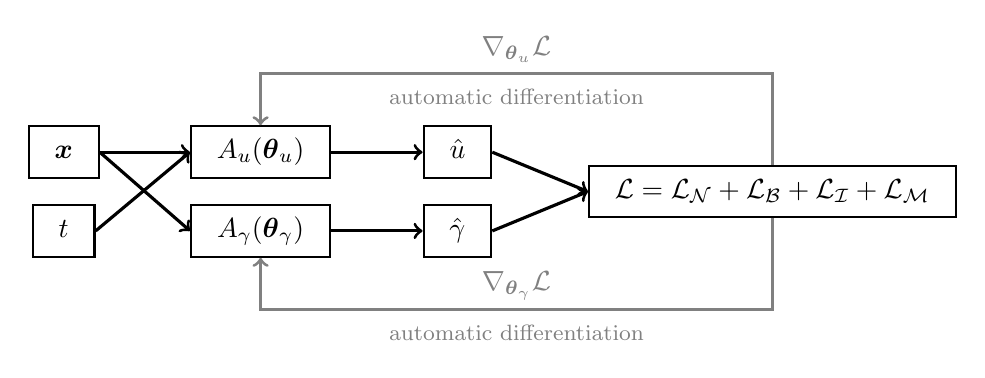
\begin{tikzpicture}
	\node (I1) [draw, thick] at (-1,0) {\begin{tabular}{c} $\boldsymbol{x}$ \end{tabular}};
	\node (I2) [draw, thick] at (-1,-1) {\begin{tabular}{c} $t$ \end{tabular}};
	\node (A1) [draw, thick] at (1.5,0) {\begin{tabular}{c} $A_u(\boldsymbol{\theta}_u)$ \end{tabular}};
	\node (A2) [draw, thick] at (1.5,-1) {\begin{tabular}{c} $A_{\gamma}(\boldsymbol{\theta}_\gamma)$ \end{tabular}};
	\node (O1) [draw, thick] at (4,0) {\begin{tabular}{c} $\hat{u}$ \end{tabular}};
	\node (O2) [draw, thick] at (4,-1) {\begin{tabular}{c} $\hat{\gamma}$ \end{tabular}};
	\node (L) [draw, thick] at (8,-0.5) {\begin{tabular}{c} $\mathcal{L}=\mathcal{L}_{\mathcal{N}}+\mathcal{L}_{\mathcal{B}}+\mathcal{L}_{\mathcal{I}}+\mathcal{L}_{\mathcal{M}}$ \end{tabular}};
	\draw [line width=0.4mm,,->] (I1.east) -- (A1.west);
	\draw [line width=0.4mm,,->] (I2.east) -- (A1.west);
	\draw [line width=0.4mm,,->] (I1.east) -- (A2.west);
	\draw [line width=0.4mm,,->] (A1.east) -- (O1.west);
	\draw [line width=0.4mm,,->] (A2.east) -- (O2.west);
	\draw [line width=0.4mm,,->] (O1.east) -- (L.west);
	\draw [line width=0.4mm,,->] (O2.east) -- (L.west);
	
	\draw [line width=0.4mm,,->,gray] (L.north) -- (8, 1) -- (1.5, 1) -- (A1.north);
	\node [gray] at (4.75,1.3) {$\nabla_{\boldsymbol{\theta}_u}\mathcal{L}$};
	\node [gray] at (4.75,0.7) {\footnotesize automatic differentiation};
	\draw [line width=0.4mm,->,gray] (L.south) -- (8, -2) -- (1.5, -2) -- (A2.south);
	\node [gray] at (4.75,-1.7) {$\nabla_{\boldsymbol{\theta}_\gamma}\mathcal{L}$};
	\node [gray] at (4.75,-2.3) {\footnotesize automatic differentiation};
	\end{tikzpicture}

\end{document}